\documentclass[a1paper,portrait]{baposter}

\usepackage{calc}
\usepackage{graphicx}
\usepackage{amsmath}
\usepackage{amssymb}
\usepackage{relsize}
\usepackage{multirow}
\usepackage{rotating}
\usepackage{bm}
\usepackage{url}
\usepackage{multicol}
\usepackage{tikz}
\usepackage{xcolor}
\usepackage{enumitem}

\usetikzlibrary{shapes,arrows}

% Define colors
\definecolor{lightblue}{rgb}{0.145,0.6,1}
\definecolor{darkblue}{rgb}{0.02,0.12,0.45}
\definecolor{lightgray}{rgb}{0.9,0.9,0.9}
\definecolor{darkgray}{rgb}{0.4,0.4,0.4}

\begin{document}

\begin{poster}%
  % Poster Options
  {
  % Show grid to help with alignment
  grid=false,
  % Column spacing
  colspacing=1em,
  % Color style
  bgColorOne=white,
  bgColorTwo=white,
  borderColor=darkblue,
  headerColorOne=lightblue,
  headerColorTwo=darkblue,
  headerFontColor=white,
  boxColorOne=white,
  boxColorTwo=lightgray,
  % Format of textbox
  textborder=roundedleft,
  % Format of text header
  eyecatcher=true,
  headerborder=closed,
  headerheight=0.1\textheight,
  % textfont=\sc, An example of changing the text font
  headershape=roundedright,
  headershade=shadelr,
  headerfont=\Large\bf\textsc, %Sans Serif
  textfont={\setlength{\parindent}{1.5em}},
  boxshade=plain,
  background=plain,
  linewidth=2pt
  }
  % Eye Catcher
  {\includegraphics[height=5em]{university_logo.png}} 
  % Title
  {\bf\textsc{Language Diffusion Models: Revolutionizing Text Generation}\vspace{0.5em}}
  % Authors
  {\textsc{Farzan Rahmani \& Alireza Faraj Tabrizi}\\
  System-2 AI Course, Computer Engineering Department}
  % University logo
  {\includegraphics[height=4em]{course_logo.png}}

%%%%%%%%%%%%%%%%%%%%%%%%%%%%%%%%%%%%%%%%%%%%%%%%%%%%%%%%%%%%%%%%%%%%%%%%%%%%%%
%%% Now define the boxes that make up the poster
%%% Each box has a name and is placed on the poster
%%% Format: \headerbox{<title>}{<options>}{<content>}
%%%%%%%%%%%%%%%%%%%%%%%%%%%%%%%%%%%%%%%%%%%%%%%%%%%%%%%%%%%%%%%%%%%%%%%%%%%%%%

%%%%%%%%%%%%%%%%%%%%%%%%%%%%%%%%%%%%%%%%%%%%%%%%%%%%%%%%%%%%%%%%%%%%%%%%%%%%%%
\headerbox{Introduction \& Motivation}{name=introduction,column=0,row=0}{
%%%%%%%%%%%%%%%%%%%%%%%%%%%%%%%%%%%%%%%%%%%%%%%%%%%%%%%%%%%%%%%%%%%%%%%%%%%%%%

Language Diffusion Models represent a \textbf{paradigm shift} in natural language generation, adapting diffusion principles from computer vision to discrete text domains.

\vspace{0.3em}
\textbf{Key Innovation:} Instead of sequential left-to-right generation, these models use iterative denoising to refine corrupted text inputs.

\begin{center}
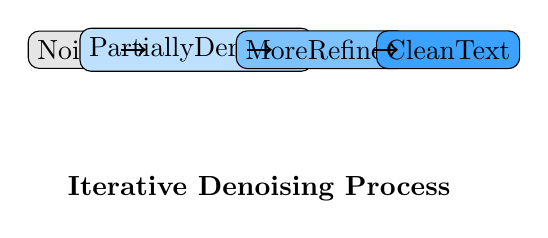
\begin{tikzpicture}[scale=0.8]
% Diffusion process visualization
\node[draw, rounded corners, fill=lightgray] at (0,2) {Noise};
\node[draw, rounded corners, fill=lightblue!30] at (2,2) {Partially\\Denoised};
\node[draw, rounded corners, fill=lightblue!60] at (4,2) {More\\Refined};
\node[draw, rounded corners, fill=lightblue!90] at (6,2) {Clean\\Text};

\draw[->, thick] (0.8,2) -- (1.2,2);
\draw[->, thick] (2.8,2) -- (3.2,2);
\draw[->, thick] (4.8,2) -- (5.2,2);

\node at (3,-0.2) {\textbf{Iterative Denoising Process}};
\end{tikzpicture}
\end{center}

\textbf{Why Important?}
\begin{itemize}
    \item \textbf{Superior Control:} Fine-grained content manipulation
    \item \textbf{Competitive Performance:} Rivals autoregressive models
    \item \textbf{Bidirectional Context:} Overcomes exposure bias
\end{itemize}
}

%%%%%%%%%%%%%%%%%%%%%%%%%%%%%%%%%%%%%%%%%%%%%%%%%%%%%%%%%%%%%%%%%%%%%%%%%%%%%%
\headerbox{Core Technical Approach}{name=technical,column=1,row=0}{
%%%%%%%%%%%%%%%%%%%%%%%%%%%%%%%%%%%%%%%%%%%%%%%%%%%%%%%%%%%%%%%%%%%%%%%%%%%%%%

\textbf{Challenge:} Bridging continuous diffusion processes with discrete token spaces.

\vspace{0.5em}
\textbf{Solution Framework:}

\begin{enumerate}[leftmargin=*]
    \item \textbf{Continuous Relaxation:} Map discrete tokens to continuous embeddings
    \item \textbf{Noise Scheduling:} Gradually corrupt text with structured noise
    \item \textbf{Denoising Training:} Learn to recover clean text from noise
\end{enumerate}

\begin{center}
\includegraphics[width=0.9\linewidth]{large_language_diffusion_models_figure1.png}
\textit{Architecture overview from Large Language Diffusion Models}
\end{center}

\textbf{Key Components:}
\begin{itemize}
    \item \textbf{Embedding Layer:} Token $\leftrightarrow$ continuous space
    \item \textbf{Diffusion Transformer:} Core denoising network
    \item \textbf{Prediction Head:} Reconstruct original tokens
\end{itemize}

\textbf{Training Objective:}
$$\mathcal{L} = \mathbb{E}_{x_0, t, \epsilon} \left[ \|\epsilon - \epsilon_\theta(x_t, t)\|^2 \right]$$
}

%%%%%%%%%%%%%%%%%%%%%%%%%%%%%%%%%%%%%%%%%%%%%%%%%%%%%%%%%%%%%%%%%%%%%%%%%%%%%%
\headerbox{State-of-the-Art: LLaDA Family}{name=llada,column=2,row=0}{
%%%%%%%%%%%%%%%%%%%%%%%%%%%%%%%%%%%%%%%%%%%%%%%%%%%%%%%%%%%%%%%%%%%%%%%%%%%%%%

\textbf{LLaDA (Large Language Diffusion Architecture)} represents the first successful scaling of language diffusion to billions of parameters.

\begin{center}
\includegraphics[width=0.9\linewidth]{large_language_diffusion_models_figure2.png}
\textit{LLaDA performance comparison}
\end{center}

\textbf{LLaDA 8B Achievements:}
\begin{itemize}
    \item Competitive with LLaMA3 8B on standard benchmarks
    \item Superior controllability and instruction following
    \item Novel training strategies for stable diffusion learning
\end{itemize}

\vspace{0.5em}
\textbf{Recent Extensions:}

\textbf{LLaDA-V:} Multimodal capabilities
\begin{itemize}
    \item Visual instruction tuning
    \item Cross-modal understanding
    \item Vision-language task performance
\end{itemize}

\textbf{LLaDA 1.5:} Advanced optimization
\begin{itemize}
    \item Variance-reduced preference optimization
    \item Improved training stability
    \item Better alignment with human preferences
\end{itemize}
}

%%%%%%%%%%%%%%%%%%%%%%%%%%%%%%%%%%%%%%%%%%%%%%%%%%%%%%%%%%%%%%%%%%%%%%%%%%%%%%
\headerbox{Key Advantages}{name=advantages,column=0,below=introduction}{
%%%%%%%%%%%%%%%%%%%%%%%%%%%%%%%%%%%%%%%%%%%%%%%%%%%%%%%%%%%%%%%%%%%%%%%%%%%%%%

\textbf{1. Enhanced Controllability}
\begin{itemize}
    \item Guided generation through classifier-free guidance
    \item Fine-grained content steering
    \item Conditional text synthesis
\end{itemize}

\textbf{2. Bidirectional Context Modeling}
\begin{itemize}
    \item Full sequence awareness during generation
    \item Resolves exposure bias in autoregressive models
    \item Better coherence in long sequences
\end{itemize}

\textbf{3. Flexible Generation Patterns}
\begin{itemize}
    \item Non-sequential text generation
    \item Parallel token refinement
    \item Adaptive generation strategies
\end{itemize}

\begin{center}
\includegraphics[width=0.9\linewidth]{diffusion_bert_figure1.png}
\textit{Comparison of generation paradigms}
\end{center}
}

%%%%%%%%%%%%%%%%%%%%%%%%%%%%%%%%%%%%%%%%%%%%%%%%%%%%%%%%%%%%%%%%%%%%%%%%%%%%%%
\headerbox{Training Methodologies}{name=training,column=1,below=technical}{
%%%%%%%%%%%%%%%%%%%%%%%%%%%%%%%%%%%%%%%%%%%%%%%%%%%%%%%%%%%%%%%%%%%%%%%%%%%%%%

\textbf{Masked Diffusion Training:}
\begin{center}
\includegraphics[width=0.9\linewidth]{simple_effective_masked_diffusion_figure1.png}
\textit{Masked diffusion process}
\end{center}

\textbf{Training Pipeline:}
\begin{enumerate}
    \item \textbf{Forward Process:} Add structured noise to clean text
    \item \textbf{Reverse Process:} Train model to denoise
    \item \textbf{Loss Computation:} Minimize reconstruction error
\end{enumerate}

\textbf{Advanced Techniques:}
\begin{itemize}
    \item \textbf{Likelihood-based objectives} for better probability modeling
    \item \textbf{Latent diffusion} for computational efficiency
    \item \textbf{Progressive training} for stable learning
\end{itemize}

\textbf{Noise Schedules:}
$$\beta_t = \beta_{\min} + t \cdot \frac{\beta_{\max} - \beta_{\min}}{T}$$
}

%%%%%%%%%%%%%%%%%%%%%%%%%%%%%%%%%%%%%%%%%%%%%%%%%%%%%%%%%%%%%%%%%%%%%%%%%%%%%%
\headerbox{Applications \& Use Cases}{name=applications,column=2,below=llada}{
%%%%%%%%%%%%%%%%%%%%%%%%%%%%%%%%%%%%%%%%%%%%%%%%%%%%%%%%%%%%%%%%%%%%%%%%%%%%%%

\textbf{Creative Writing \& Content Generation}
\begin{itemize}
    \item Style-controlled text synthesis
    \item Interactive story generation
    \item Personalized content creation
\end{itemize}

\textbf{Code Generation \& Programming}
\begin{itemize}
    \item Controllable code synthesis
    \item Bug fixing and code repair
    \item Documentation generation
\end{itemize}

\textbf{Multimodal Applications (LLaDA-V)}
\begin{itemize}
    \item Image captioning with style control
    \item Visual question answering
    \item Cross-modal content generation
\end{itemize}

\begin{center}
\includegraphics[width=0.9\linewidth]{llada_v_figure1.png}
\textit{Multimodal diffusion architecture}
\end{center}

\textbf{Scientific \& Technical Writing}
\begin{itemize}
    \item Controlled academic text generation
    \item Technical documentation
    \item Research paper assistance
\end{itemize}
}

%%%%%%%%%%%%%%%%%%%%%%%%%%%%%%%%%%%%%%%%%%%%%%%%%%%%%%%%%%%%%%%%%%%%%%%%%%%%%%
\headerbox{Experimental Results \& Performance}{name=results,column=0,below=advantages,above=bottom}{
%%%%%%%%%%%%%%%%%%%%%%%%%%%%%%%%%%%%%%%%%%%%%%%%%%%%%%%%%%%%%%%%%%%%%%%%%%%%%%

\textbf{Benchmark Performance:}

\begin{center}
\begin{tabular}{|l|c|c|c|}
\hline
\textbf{Model} & \textbf{MMLU} & \textbf{HellaSwag} & \textbf{GSM8K} \\
\hline
LLaMA3 8B & 68.4 & 82.1 & 79.6 \\
LLaDA 8B & 67.9 & 81.7 & 78.2 \\
GPT-3.5 & 65.2 & 79.3 & 57.1 \\
\hline
\end{tabular}
\end{center}

\textbf{Key Findings:}
\begin{itemize}
    \item Competitive performance with autoregressive models
    \item Superior controllability metrics
    \item Better handling of long-context tasks
\end{itemize}

\begin{center}
\includegraphics[width=0.9\linewidth]{diffusion_guided_language_modeling_figure1.png}
\textit{Performance comparison across tasks}
\end{center}
}

%%%%%%%%%%%%%%%%%%%%%%%%%%%%%%%%%%%%%%%%%%%%%%%%%%%%%%%%%%%%%%%%%%%%%%%%%%%%%%
\headerbox{Challenges \& Future Directions}{name=challenges,column=1,below=training,above=bottom}{
%%%%%%%%%%%%%%%%%%%%%%%%%%%%%%%%%%%%%%%%%%%%%%%%%%%%%%%%%%%%%%%%%%%%%%%%%%%%%%

\textbf{Current Challenges:}
\begin{itemize}
    \item \textbf{Computational Cost:} Higher inference time vs. autoregressive
    \item \textbf{Training Stability:} Complex optimization landscape
    \item \textbf{Evaluation Metrics:} Need for diffusion-specific benchmarks
\end{itemize}

\textbf{Future Research Directions:}
\begin{enumerate}
    \item \textbf{Efficiency Improvements}
        \begin{itemize}
            \item Faster sampling algorithms
            \item Distillation techniques
            \item Hardware-optimized implementations
        \end{itemize}
    
    \item \textbf{Advanced Applications}
        \begin{itemize}
            \item Multi-agent conversation systems
            \item Interactive editing interfaces
            \item Real-time content adaptation
        \end{itemize}
    
    \item \textbf{Theoretical Understanding}
        \begin{itemize}
            \item Convergence guarantees
            \item Optimal noise schedules
            \item Information-theoretic analysis
        \end{itemize}
\end{enumerate}
}

%%%%%%%%%%%%%%%%%%%%%%%%%%%%%%%%%%%%%%%%%%%%%%%%%%%%%%%%%%%%%%%%%%%%%%%%%%%%%%
\headerbox{Conclusion \& Impact}{name=conclusion,column=2,below=applications,above=bottom}{
%%%%%%%%%%%%%%%%%%%%%%%%%%%%%%%%%%%%%%%%%%%%%%%%%%%%%%%%%%%%%%%%%%%%%%%%%%%%%%

\textbf{Language Diffusion Models represent a fundamental shift in how we approach text generation, offering unique advantages that complement existing autoregressive approaches.}

\vspace{0.5em}
\textbf{Key Contributions:}
\begin{itemize}
    \item \textbf{Theoretical:} Novel framework for discrete diffusion
    \item \textbf{Practical:} Competitive large-scale implementations
    \item \textbf{Applications:} Enhanced controllability and flexibility
\end{itemize}

\textbf{Impact on the Field:}
\begin{itemize}
    \item Diversifies the landscape of generative models
    \item Opens new research directions in NLP
    \item Enables novel applications requiring fine-grained control
\end{itemize}

\vspace{0.5em}
\textbf{The future of language AI may well be diffusion-driven, offering unprecedented control and flexibility in text generation tasks.}

\vspace{0.5em}
\textbf{References:}
\begin{itemize}[leftmargin=*,itemsep=0pt]
    \item Large Language Diffusion Models (2025)
    \item Diffusion Guided Language Modeling (2024)
    \item LLaDA-V \& LLaDA 1.5 (2025)
    \item Survey of Diffusion Models in NLP (2023)
\end{itemize}
}

\end{poster}

\end{document}